\subsection{Direct Detection}
After executing the flavour processes where the NP states had the role of mediators, we now turn towards the phenomenological aspects of DM itself.
We begin with direct detection (DD) or nucleon scattering where a DM particle scatters off a parton (quark or gluon) of a nucleon. 
\\ \\ \textit{Effective Lagrangian}\\
This can happen
due to a spin independent (SI) or spin dependent (SD) interaction \eqref{eq_th.sigma.dd} which are described by an effective Lagrangian (1104.0228)
\begin{align}
 \mathcal{L}^\text{eff} = \sum\limits_{q} \mathcal{L}^\text{eff}_q + \mathcal{L}^\text{eff}_g.
\end{align}
We use $q$ for the light quarks $u$, $d$, $s$ and $Q$ for heavier $c$, $b$, $t$. From \eqref{eq_fierzSPtoVA} we see that from our chiral model, 
we only get effective interactions with quarks like $\bar \chi\gamma\mu\chi \bar q\gamma_\mu q$ and $\bar \chi\gamma^\mu\gamma_5 \bar q\gamma_\mu \gamma_5 q$
as six dimensional operators. The former vanishes for Majorana DM and the latter is SD which will not give stronger constraints than the following SI
interactions but the resulting SD cross section can be evaluated with the expressions also given in (1104.0228) for the leading processes to be of
order $\mathcal{O}(10^{-44})$ cm$^2$ while the upper limits obtained by IceCube (1301.6620 or direct source) yield $\mathcal{O}(10^{-40})$ cm$^2$ for 
a 100 GeV'ish DM particle.
So we neglect them. A possibly occuring scalar operator $\bar \chi \chi \bar q q$ also vanishes in our chiral model. Therefore the first contributing
SI operators coming from quark interactions are eight dimensional, namely those depending on twist-2 operators. They are the traceless parts of the
quark energy momentum tensor and arise from the matrix element of a quark current product expressed in local operators (MDSchwartz). The twist of 
an operator is the difference of its mass dimension and its spin. So much for the quark interaction. Since our DM particle shall be an 
$SU(3)_C$-singlet, it does not couple directly to gluons $g$ but scalarlike at one-loop level through the heavy quarks. There is also a twist-2 
operator for the gluon but its coefficient will be suppressed by $\alpha_s$ so we will not consider it further. So at least for our $SU(2)_L$ singlet
DM particle which does not interact with the $W$ bosons, the leading SI Lagrangian is
%For both DM $SU(2)_L$-representations, the singlet and the triplet, the leading SI operators are
\begin{align}
 \mathcal{L}^\text{eff} =&\, \frac{g_q^{(1)}}{m_\chi} \bar \chi\ti \partial_\mu \gamma_\nu O_q^{\mu\nu} + \frac{g_q^{(2)}}{m^2_\chi} \bar \chi(\ti \partial_\mu) (\ti\partial_\nu) O_q^{\mu\nu} \\
 \nonumber
 &+ f_G \bar \chi \chi G^a_{\mu\nu} G^{a\mu\mu}.
\end{align}
The twist-2 operator for the quark is
\begin{align}
 O_q^{\mu\nu} = \frac12 \bar q \ti \left(D^\mu \gamma^\nu + D^\nu \gamma^\mu - \frac12 g^{\mu\nu} \slashed{D}\right) q
\end{align}
and the three coefficients of mass dimension $-3$ $g_q^{(1)}$, $g_q^{(2)}$ and $f_G$ enter the form factor $f_N$ in \eqref{eq_th.sigma.dd} as
\begin{align}
 \frac{f_N}{m_N} = \sum\limits_{q,c,b} \frac34 \left(q(2)+\bar q(2)\right) \left(g_q^{(1)} + g_q^{(2)}\right) - \frac{8\pi}{9\alpha_s}f_{TG}f_G
 \label{eq_ddformfactorA}
\end{align}
where the matrix elements of the effective operators are expressed with the nucleon mass $m_N$ as (1007.2601)
\begin{subequations}
\begin{align}
 \langle N(p)| O_q^{\mu\nu} | N(p)\rangle =& \frac{1}{m_N}\left(p^\mu p^\nu - \frac14 m_N^2 g^{\mu\nu}\right) \left(q(2) + \bar q(2)\right),\\
 f_{TG} :=& 1- \sum\limits_q f_{Tq},\\
 f_{Tq} :=& \langle N|m_n \bar qq |N\rangle /m_N.
\end{align}
\end{subequations}
The quantities $q(2)$ and $\bar q(2)$ are the second moments (0811.1779) of the parton distribution function (PDF) of quark $q(x)$ or antiquark 
$\bar q(x)$, respectively, in the nucleon $q(2)+\bar q(2) = \int_0^1 \dx x^2 \left[q(x) + \bar q(x)\right]$. The values used for the numerical
calculation are listed in tabular \ref{tab_parton}.
\begin{table}[b]
 \begin{tabular}{c|ccccc}
   & $u$ & $d$ & $s$ & $c$ &$b$ \\
   \hline
  $q(2)$ & 0.22 & 0.11 & 0.026 & 0.019 & 0.012\\
  $\bar q(2)$ & 0.034 & 0.036 & 0.026 & 0.019 & 0.012\\
  $f_{Tq}$ & 0.020& 0.026 & 0.134 (1209.3641)\\
 \end{tabular}
\caption{Second moments $q(2)$, $\bar q(2)$ of the quark PDFs evaluated at $\mu=m_Z$ and taken from (CITE) and scalar matrix elements $f_{Tq}$ of 
the light quarks for the 
proton each. For the neutron $u(2)$ and $d(2)$ just swap and $f_{Tu}$ and $f_{Td}$ differ slightly (CITE). All other quantities are the same. }
\label{tab_parton}
\end{table}
\noindent The evaluation of $f_G$ is factorised in a ``short distance'' (SD, not to confuse with spin dependent) and a ``long distance'' (LD) 
contribution
\begin{align}
 f_G|_q = f_G|^\text{SD}_q + f_G|^\text{LD}_q. 
\end{align}
The former (latter) represents a scale of heavy (light) particles as the colored scalar mediator (quarks). While we need to calculate the full
loop process e.g. in figure \ref{fig_quarkgluon.eps} for the SD, the LD with $Q$ can be thought of a triangle diagram where $\Phi_q$ integrated 
out i.e. there arises a four fermion operator $f_Q m_Q \bar \chi \bar Q Q$. The triangle loop calculation yields in the heavy scalar mass limit 
\begin{align}
 f_G|_Q^\text{LD} = -\frac{\alpha_s}{12\pi} c_Q f_Q,
\end{align}
with $c_Q = 1+11\alpha_s(m_Q)/4\pi$ coming from large QCD corrections (CITE DjoUadi Drees), $c_c=1.32$, $c_b = 1.19$, $c_t = 1$.
When considering the light quarks $q$ in the LD term, they have a vanishing contribution since the respective operator goes with the quark mass
which is each smaller than $\Lambda_\text{QCD} = \mathcal{O}(100)$ MeV and their propagators are entirely determined by confinement dynamics. Thus,
we do not have to take them into account. The explicit formula for the operator coefficients \eqref{eq_ddformfactorA} for the singlet case 
will be given now
\\ \\ \textit{Singlet Dark Matter}\\
bla



\begin{figure}[t]
 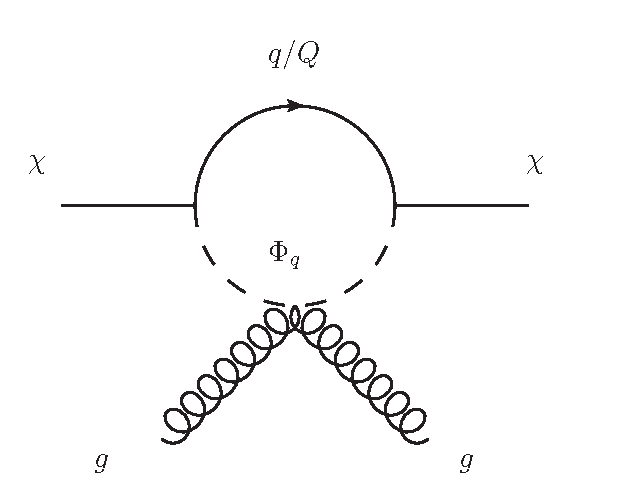
\includegraphics[width=0.5\textwidth]{../pics/phigluon.eps}
\end{figure}


